\documentclass[12pt, letterpaper]{article}
\usepackage[utf8]{inputenc}
\usepackage{fancyhdr}
\usepackage{graphicx}
\usepackage{float}
\graphicspath{ {./images/} }
\usepackage[hidelinks]{hyperref}
\usepackage{wasysym}

% Title Page
\title{Software Development Project - 1DV600 - Test documentation}
\author{Claes Weyde \\ 
	e-mail: \href{mailto:cw222av@student.lnu.se}{cw222av@student.lnu.se} \\
	github: \href{https://github.com/Cosbus/cw222av_1dv600_}{https://github.com/Cosbus/\texttt{cw222av\_1dv600\_}}}

\pagestyle{fancy}
\fancyhf{}
\fancyhead[R]{The Marvelous Hanging Man - Test documentation}
\fancyhead[L]{Claes Weyde}
\fancyfoot[C,C]{\leftmark}
\fancyfoot[L]{\thepage}
\fancyfoot[R]{Version 1.0}



\begin{document}
\maketitle
\newpage
\tableofcontents{}
\newpage

\section{Test Plan}

\subsection{Objectives}
The objective of this testing phase is to snuff out as many problems with the application as possible. The testing is aimed at making sure the critical system functions are operational. As this is primarily a game, a large focus is put on the gaming part to make sure that it is working properly. However, since the words used in the game are of great importance to minimize repetitiveness quite a large focus is put on the functionality regarding adding, deleting and updating the words.
\subsubsection{What to test?}
As was described above the main testing will be performed on the gaming part of the application. Manual test will be performed to determine that all the critical functionality works with regards to game play, specifically UC2 - Play game (UC 1 is concerned with the main menu and is not tested here). The main scenario as well as some alternative scenarios will be tested.
\begin{itemize}
	\item Choosing a game difficulty.
	\item Providing a letter successfully and unsuccessfully.
	\item Quitting the game.
	\item Finishing a word.
\end{itemize}
Some attention will also be put on managing words, i.e. UC 5, 6 and 7. All of the manual dynamic tests are to be performed after the code for the use cases have been implemented. For a full breakdown of the manual testing please see section \ref{matrix}.
\newline
\newline
Automated unit tests will also be written to test some of the methods provided in the different objects of the application.
\subsection{To-do}
\begin{itemize}
	\item Study course material regarding testing
	\item Manual TC - planning
	\item Manual TC - perform
	\item Automated unit test - planning (including learning frameworks etc.)
	\item Automated unit test - perform
	\item Test report
\end{itemize}
\subsection{Time estimates and Time log}
\begin{center}
	\begin{tabular}{|c|c|c|} 
		\hline
		Task & Estimate [hrs] & Actual time \\ [0.5ex] 
		\hline\hline
		Study course material regarding testing & 5 & 3 \\ 
		\hline
		Manual TC - planning & 2 & 2.5 \\
		\hline 
		Manual TC - perform & 0.5 & 0.5 \\ 
		\hline
		Automated unit test - planning & 4 & 3.5 \\ 
		\hline 		
		Automated unit test - perform & 4 & 2.5 \\
		\hline
		Test report & 2 & 2.5 \\
		\hline
		Total time & 17.5 & 14.5\\ [1ex]
		\hline
		
	\end{tabular}
\end{center}
\newpage
\section{Manual test cases}
\subsection{Manual tests of Play Game main scenario}
\subsubsection{TC 2.2 - Successfully providing a correct letter}
\begin{itemize}
	\item Name: Successfully providing a correct letter.
	\item Test case ref: TC 2.2
	\item Use case ref: UC 2
	\item Description: The test case tests how the system responds when the user provides a letter which is correct, and the word is not completely solved.
\end{itemize}
\emph{Input}
\begin{enumerate}
	\item \underline{Precondition:} The user has started the game.
	\item Test case TC 2.1. choose "play game" from main menu.
	\item Input a correct letter.
	\item Press enter.
\end{enumerate}
\emph{Expected}
\begin{itemize}
	\item The system prints "Correct!" on the screen.
	\item The system prints the number of letters remaining on the screen.
	\item The system prints the number of tries remaining on the screen.
	\item The system prompts the user to enter a new letter by printing "Please provide a letter:" on the screen.
\end{itemize}
\begin{Form}
	\CheckBox{Test successful}
	\newline
	\CheckBox{Test not successful}
	\newline
\end{Form}
\newline
\emph{Comments}
\newline
\newline
\newline
\newline
\newline
\newline
\newline
\subsubsection{TC 2.3 - Providing an incorrect letter}
\begin{itemize}
	\item Name: Providing an incorrect letter.
	\item Test case ref: TC 2.3
	\item Use case ref: UC 2
	\item Description: The test case tests how the system responds when the user provides a letter which is incorrect, and the user has more tries.
\end{itemize}
\emph{Input}
\begin{enumerate}
	\item \underline{Precondition:} The user has started the game.
	\item Test case TC 2.1. choose "play game" from main menu.
	\item Input an incorrect letter.
	\item Press enter.
\end{enumerate}
\emph{Expected}
\begin{itemize}
	\item The system prints "Unfortunately wrong." on the screen.
	\item The system prints the number of letters remaining on the screen.
	\item The system prints the number of tries remaining on the screen.
	\item The system prompts the user to enter a new letter by printing "Please provide a letter:" on the screen.
\end{itemize}
\begin{Form}
	\CheckBox{Test successful}
	\newline
	\CheckBox{Test not successful}
	\newline
\end{Form}
\newline
\emph{Comments}
No problems detected.
\subsubsection{TC 2.6 - Returning from play to main menu}
\begin{itemize}
	\item Name: Returning from play to main menu.
	\item Test case ref: TC 2.6
	\item Use case ref: UC 2
	\item Description: The test case tests how the system responds when the user has finished a word (either by finding the word or having exhausted his/hers amount of tries) and chooses to return to the main menu.
\end{itemize}
\emph{Input}
\begin{enumerate}
	\item \underline{Precondition:} The user has finished a word and the system has provided the user with the choice of returning to main menu, playing a new word or quitting the game altogether.
	\item Finish a word.
	\item Input "m" to return to main menu.
	\item Press enter.
\end{enumerate}
\emph{Expected}
\begin{itemize}
	\item The system shows the main menu on the screen.
\end{itemize}
\begin{Form}
	\CheckBox{Test successful}
	\newline
	\CheckBox{Test not successful}
	\newline
\end{Form}
\newline
\emph{Comments}
No problems encountered.
\subsubsection{TC 2.a* - Quitting the game while playing}
\begin{itemize}
	\item Name: Quitting the game while playing.
	\item Test case ref: TC 2.a*
	\item Use case ref: UC 2
	\item Description: The test case tests how the system responds when the user enters the code for quitting the game while playing.
\end{itemize}
\emph{Input}
\begin{enumerate}
	\item \underline{Precondition:} The user is playing the game.
	\item Input "q-t" and press enter.
	\item The system asks the user if he/she really wants to quit.
	\item Input "y" and press enter.
\end{enumerate}
\emph{Expected}
\begin{itemize}
	\item The system quits the application entirely.
\end{itemize}
\begin{Form}
\CheckBox{Test successful}
\newline
\CheckBox{Test not successful}
\newline
\end{Form}
\newline
\emph{Comments}
No problems encountered.
\subsubsection{TC 3.1 - Moving to managing words menu}
\begin{itemize}
	\item Name: Authenticating for managing words.
	\item Test case ref: TC 3.1
	\item Use case ref: UC 3
	\item Description: The test case tests how the system responds when the user tries to open the "manage words" menu.
\end{itemize}
\emph{Input}
\begin{enumerate}
	\item \underline{Precondition:} The user is located in the main menu.
	\item Select "Manage word." by using the cursor keys.
	\item Press enter.
\end{enumerate}
\emph{Expected}
\begin{itemize}
	\item The system prints "You need to be authenticated to manage words."
	\item The system prompts the user to "Input password:"
\end{itemize}
\begin{Form}
	\CheckBox{Test successful}
	\newline
	\CheckBox{Test not successful}
	\newline
\end{Form}
\newline
\emph{Comments}
No problems encountered.
\subsubsection{TC 3.2 - Inputting an incorrect password}
\begin{itemize}
	\item Name: Inputting an incorrect password.
	\item Test case ref: TC 3.2
	\item Use case ref: UC 3
	\item Description: The test case tests how the system responds when the user tries inputs an incorrect password when prompted for a password to move to the "manage words" menu.
\end{itemize}
\emph{Input}
\begin{enumerate}
	\item \underline{Precondition:} The user has selected "manage words" from the main menu and have been prompted by the system to input a password.
	\item Write "Frog"
	\item Press enter.
\end{enumerate}
\emph{Expected}
\begin{itemize}
	\item The system prints "Unfortunately the password was incorrect"
	\item The system displays the main menu.
\end{itemize}
\begin{Form}
	\CheckBox{Test successful}
	\newline
	\CheckBox{Test not successful}
	\newline
\end{Form}
\newline
\emph{Comments}
No problems encountered.
\subsubsection{TC 3.3 - Inputting a correct password}
\begin{itemize}
	\item Name: Inputting a correct password.
	\item Test case ref: TC 3.3
	\item Use case ref: UC 3
	\item Description: The test case tests how the system responds when the user tries inputs a correct password when prompted for a password to move to the "manage words" menu.
\end{itemize}
\emph{Input}
\begin{enumerate}
	\item \underline{Precondition:} The user has selected "manage words" from the main menu and have been prompted by the system to input a password.
	\item Write "deconstructor"
	\item Press enter.
\end{enumerate}
\emph{Expected}
\begin{itemize}
	\item The system displays the "Manage Words" menu.
\end{itemize}
\begin{Form}
	\CheckBox{Test successful}
	\newline
	\CheckBox{Test not successful}
	\newline
\end{Form}
\newline
\emph{Comments}
No problems encountered.

\subsubsection{TC 5.3 - Inputting a new word}
\begin{itemize}
	\item Name: Inputting a new word.
	\item Test case ref: TC 5.3
	\item Use case ref: UC 5
	\item Description: The test case tests how the system responds when the user enters a new word to save to the word list.
\end{itemize}
\emph{Input}
\begin{enumerate}
	\item \underline{Precondition:} The user has moved to the manage words menu and chosen to add a new word. The system prompts the user to input the word by printing "Input a word:" on the screen.
	\item Input a word and press enter.
\end{enumerate}
\emph{Expected}
\begin{itemize}
	\item The system prints "Make a choice: (use arrow keys)".
	\item The system prints the three difficulty levels "easy", "moderate" and "hard" which the user can move between.
\end{itemize}
\begin{Form}
\CheckBox{Test successful}
\newline
\CheckBox{Test not successful}
\newline
\end{Form}
\newline
\emph{Comments}
Works as expected.
\subsubsection{TC 5.5 - Choosing a difficulty for an input word}
\begin{itemize}
	\item Name: Choosing a difficulty for an input word.
	\item Test case ref: TC 5.5
	\item Use case ref: UC 5
	\item Description: The test case tests how the system responds when the user enters a difficulty for an input word.
\end{itemize}
\emph{Input}
\begin{enumerate}
	\item \underline{Precondition:} The user has input a word and pressed enter.
	\item TC 5.3. Choose a difficulty presented by the system.
	\item Press enter.
\end{enumerate}
\emph{Expected}
\begin{itemize}
	\item The system prints "Successfully saved" in green text.
	\item The system prints "Add another word? [y/n]" and waits for the user to respond.
\end{itemize}
\begin{Form}
\CheckBox{Test successful}
\newline
\CheckBox{Test not successful}
\newline
\end{Form}
\newline
\emph{Comments}
No problems found.
\subsubsection{TC 6.2 - Choosing to remove a word}
\begin{itemize}
	\item Name: Choosing to remove a word.
	\item Test case ref: TC 6.2
	\item Use case ref: UC 6
	\item Description: The test case tests how the system responds when the user chooses to remove a word.
\end{itemize}
\emph{Input}
\begin{enumerate}
	\item \underline{Precondition:} The user has moved to the manage words menu and the system has printed the menu on the screen.
	\item Choose to remove a word by moving the cursor to the "delete word" choice using the arrow keys.
	\item Press enter.
\end{enumerate}
\emph{Expected}
\begin{itemize}
	\item The system prints "Remove word. What difficulty are you interested in" on the screen.
	\item The system prints "Make a choice: (use arrow keys)" on the screen.
	\item The system prints the choices "easy", "moderate" and "hard" on the screen and waits for the user choice.
\end{itemize}
\begin{Form}
	\CheckBox{Test successful}
	\newline
	\CheckBox{Test not successful}
	\newline
\end{Form}
\newline
\emph{Comments}
Works, the word has been removed.
\subsubsection{TC 6.3.1 - Choosing a difficulty for the word to remove}
\begin{itemize}
	\item Name: Choosing a difficulty for the word to remove.
	\item Test case ref: TC 6.3.1
	\item Use case ref: UC 6
	\item Description: The test case tests how the system responds when the user chooses a difficulty for the word to be removed.
\end{itemize}
\emph{Input}
\begin{enumerate}
	\item \underline{Precondition:} The user has chosen to remove a word (TC 6.2).
	\item Choose a difficulty and press enter.
\end{enumerate}
\emph{Expected}
\begin{itemize}
	\item The system prints all the words on file for the given difficulty on the screen and waits for the user choice. The user can move between the words using the arrow keys to choose.
\end{itemize}
\begin{Form}
	\CheckBox{Test successful}
	\newline
	\CheckBox{Test not successful}
	\newline
\end{Form}
\newline
\emph{Comments}
Works.
\subsubsection{TC 6.3.2 - Choosing a word to remove from the list}
\begin{itemize}
	\item Name: Choosing a word to remove from the list.
	\item Test case ref: TC 6.3.2
	\item Use case ref: UC 6
	\item Description: The test case tests how the system responds when the user chooses a word from the list to remove.
\end{itemize}
\emph{Input}
\begin{enumerate}
	\item \underline{Precondition:} The user has chosen a difficulty for the word to remove (TC 6.3.1).
	\item Choose a word from the list by using the arrow keys.
	\item Press enter.
\end{enumerate}
\emph{Expected}
\begin{itemize}
	\item The system prints "Are you sure you want to remove "[thechoosenword]" [y/n]?" and awaits the users answer.
\end{itemize}
\begin{Form}
	\CheckBox{Test successful}
	\newline
	\CheckBox{Test not successful}
	\newline
\end{Form}
\newline
\emph{Comments}
No problems.
\subsubsection{TC 6.3.2a - Confirming removal of a chosen word}
\begin{itemize}
	\item Name: Confirming removal of a chosen word.
	\item Test case ref: TC 6.3.2a
	\item Use case ref: UC 6
	\item Description: The test case tests how the system responds when the user confirms removal of the chosen word.
\end{itemize}
\emph{Input}
\begin{enumerate}
	\item \underline{Precondition:} The user has chosen a word to remove from the list (TC 6.3.2).
	\item Write "y".
	\item Press enter.
\end{enumerate}
\emph{Expected}
\begin{itemize}
	\item The system prints "[word] successfully removed!" in green text.
	\item The system prints "Delete another word? [y/n]" and awaits the user response.
\end{itemize}
\begin{Form}
	\CheckBox{Test successful}
	\newline
	\CheckBox{Test not successful}
	\newline
\end{Form}
\newline
\emph{Comments}
No problems.
\subsubsection{TC 6.3.2b - Not confirming to remove a chosen word}
\begin{itemize}
	\item Name: Not confirming to remove a chosen word.
	\item Test case ref: TC 6.3.2b
	\item Use case ref: UC 6
	\item Description: The test case tests how the system responds when the user chooses to not confirm to remove a word chosen for removal.
\end{itemize}
\emph{Input}
\begin{enumerate}
	\item \underline{Precondition:} The user has chosen a word to remove from the list (TC 6.3.2).
	\item Write "n".
	\item Press enter.
\end{enumerate}
\emph{Expected}
\begin{itemize}
	\item The system prints "Maybe a wise choice?".
	\item The system prints "Do you want to remove another word [y/n]? and awaits the users answer.
\end{itemize}
\begin{Form}
	\CheckBox{Test successful}
	\newline
	\CheckBox{Test not successful}
	\newline
\end{Form}
\newline
\emph{Comments}
Not successful. The system moves back to the choice of choosing a difficulty to remove. When continuing the system goes haywire after a while. It would seem that the system emits new events while not removing old ones. This must be taken care of.
\subsubsection{TC 7.3 - Choosing a word to update}
\begin{itemize}
	\item Name: Choosing a word to update.
	\item Test case ref: TC 7.3
	\item Use case ref: UC 7
	\item Description: The test case tests how the system responds when the user chooses a word to update.
\end{itemize}
\emph{Input}
\begin{enumerate}
	\item \underline{Precondition:} The user has chosen to update a word from the manage word menu and chosen which difficulty the word should belong to (TC 7.2).
	\item Choose a word by using the arrow keys.
	\item Press enter.
\end{enumerate}
\emph{Expected}
\begin{itemize}
	\item The system prints "What word do you want to update "[word]" to?".
	\item The system awaits the user choice.
\end{itemize}
\begin{Form}
	\CheckBox{Test successful}
	\newline
	\CheckBox{Test not successful}
	\newline
\end{Form}
\newline
\emph{Comments}
Works.
\subsubsection{TC 7.5 - Choosing a word to update to}
\begin{itemize}
	\item Name: Choosing a word to update to.
	\item Test case ref: TC 7.5
	\item Use case ref: UC 7
	\item Description: The test case tests how the system responds when the user inputs a word to update to.
\end{itemize}
\emph{Input}
\begin{enumerate}
	\item \underline{Precondition:} The user has chosen a word to update from the list of words (TC 7.2).
	\item Write the word to update to.
	\item Press enter.
\end{enumerate}
\emph{Expected}
\begin{itemize}
	\item The system prints "Are you sure you want to update "[oldword]" to "[newword]" [y/n]?" and awaits the user answer.
\end{itemize}
\begin{Form}
	\CheckBox{Test successful}
	\newline
	\CheckBox{Test not successful}
	\newline
\end{Form}
\newline
\emph{Comments}
Works.
\subsubsection{TC 7.6 - Answering with wrong letter to [y/n] question}
\begin{itemize}
	\item Name: Answering with wrong letter to [y/n] question.
	\item Test case ref: TC 7.6
	\item Use case ref: UC 7
	\item Description: The test case tests how the system responds when the user answers with an un-allowed letter to a yes/no question when updating words.
\end{itemize}
\emph{Input}
\begin{enumerate}
	\item \underline{Precondition:} The user has entered a word to update to (TC 7.5).
	\item Write any letter or number which differs from "y" or "n".
	\item Press enter.
\end{enumerate}
\emph{Expected}
\begin{itemize}
	\item The system prints "Please answer "y" or "n"!".
	\item The system prints "Are you sure you want to update "[oldword]" to "[newword]" [y/n]?" and awaits the user answer.
\end{itemize}
\begin{Form}
	\CheckBox{Test successful}
	\newline
	\CheckBox{Test not successful}
	\newline
\end{Form}
\newline
\emph{Comments}
Works.
\section{Automated tests}
The unit test cover a class called authenticator to authenticate if the user can manage words, a class called FileHandler which handles the saving and loading of words for a given game, and a class called Word which handles a single word in the wordlist. The frameword Mocha together with Chai and Chai-as-promised (for testing asynchronous methods) was used for performing automated testing in Node.js.
\subsection{Test runs}
 A screenshot of the output from the automated tests can be found in figure \ref{fig:automatedTest1}. As can be seen from figure \ref{fig:automatedTest1}, the method getSumAndQ in the Authenticator class fails for a certain scenario. Figure \ref{fig:automatedTest2} show a new test-run performed after having fixed the bug in the code. As can be seen, all test now succeed. 
\newline
\begin{figure}[H]\label{fig:automatedTest1}
	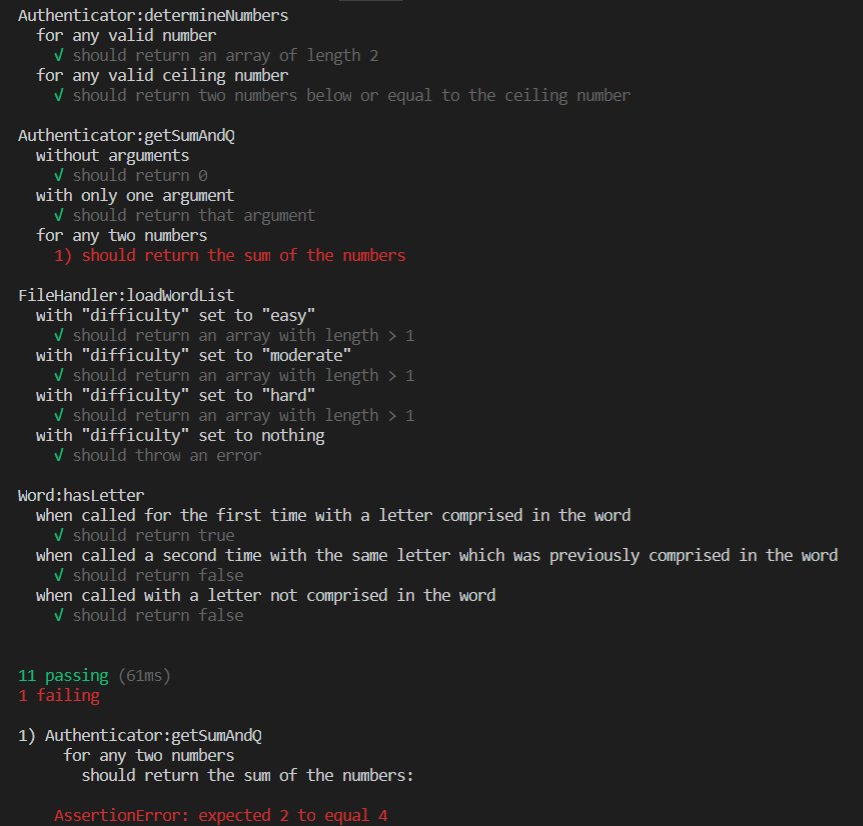
\includegraphics{automatedTest1}
	\caption{Automated test run with a bug in the code.}
	\centering
\end{figure}
\begin{figure}[H]\label{fig:automatedTest2}
	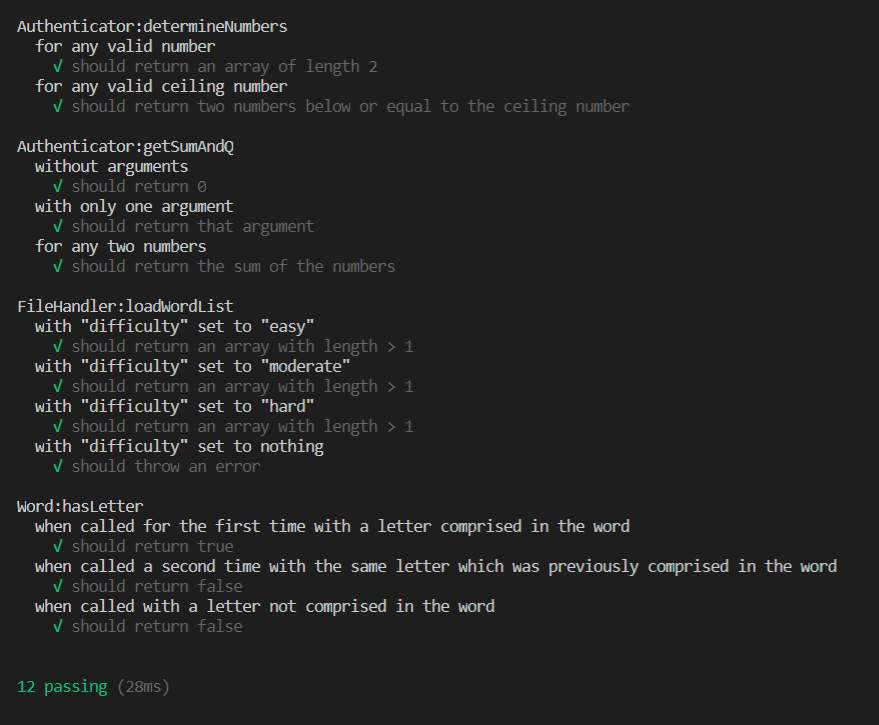
\includegraphics{automatedTest2}
	\caption{Automated test run with the bug removed.}
	\centering
\end{figure}
\subsection{The test code}
The test code can be found in the figures below. Three files were used, one for each class tested (due to space constraints there are two screenshots for each test file).
\begin{figure}[H]\label{fig:code11}
	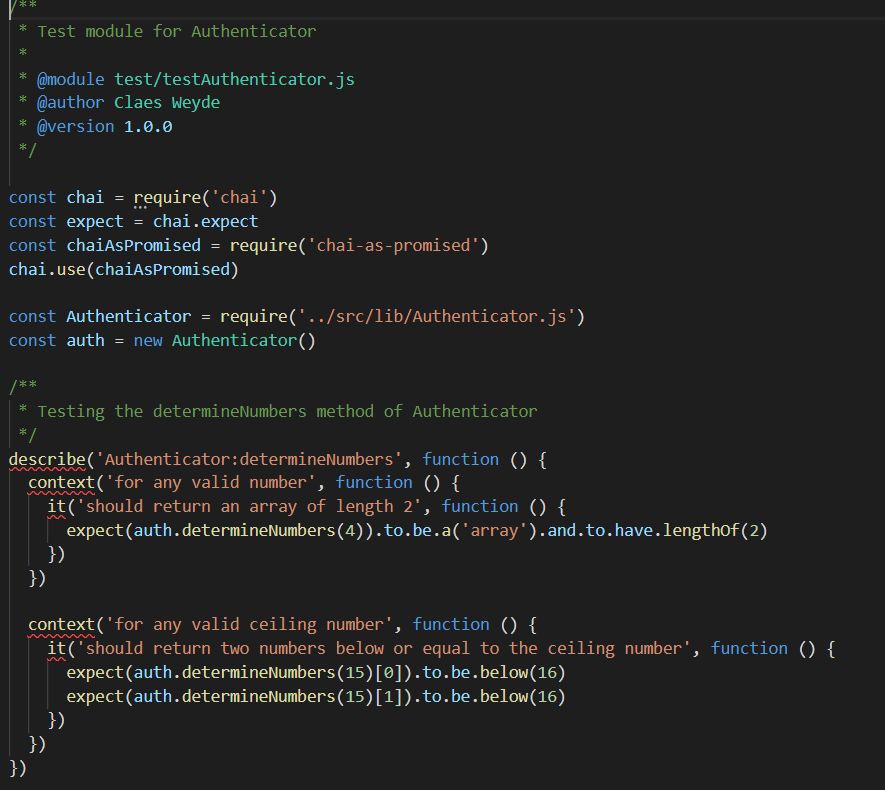
\includegraphics{code1_1}
	\caption{Test code for Authenticator 1 of 2}
	\centering
\end{figure}
\begin{figure}[H]\label{fig:code12}
	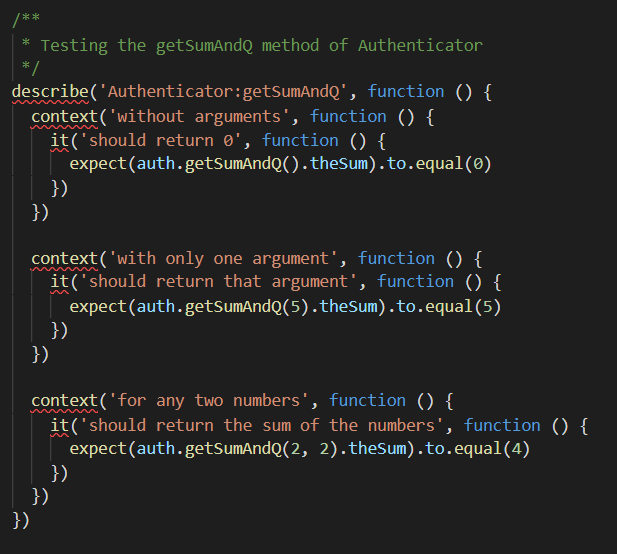
\includegraphics{code1_2}
	\caption{Test code for Authenticator 2 of 2}
	\centering
\end{figure}
\begin{figure}[H]\label{fig:code21}
	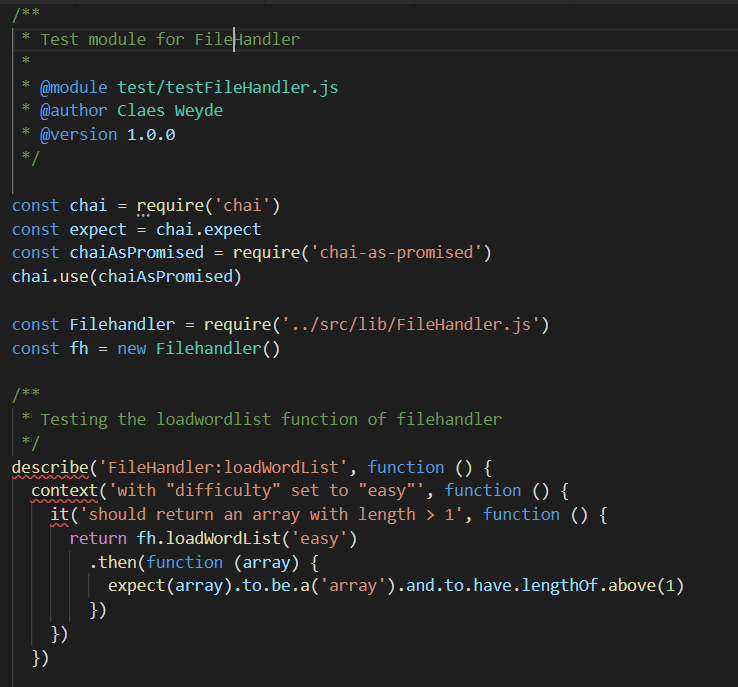
\includegraphics{code2_1}
	\caption{Test code for FileHandler 1 of 2}
	\centering
\end{figure}
\begin{figure}[H]\label{fig:code22}
	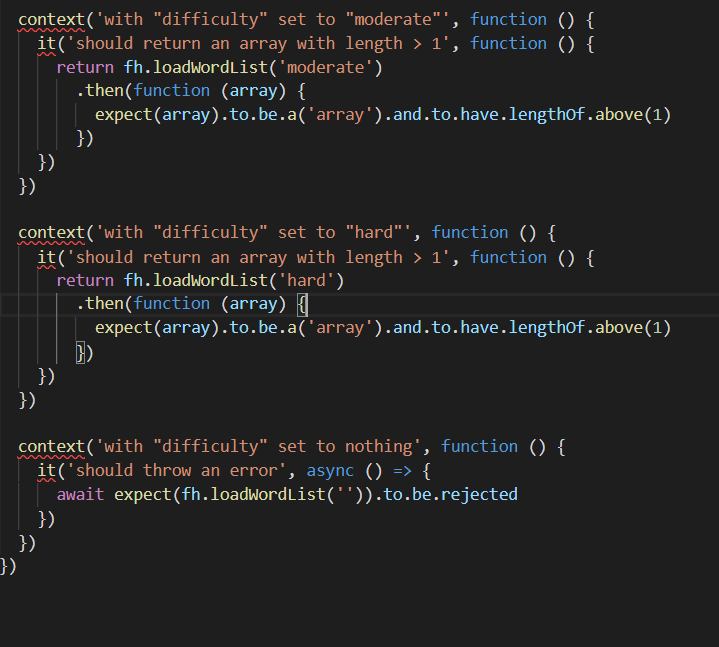
\includegraphics{code2_2}
	\caption{Test code for FileHandler 2 of 2}
	\centering
\end{figure}
\begin{figure}[H]\label{fig:code31}
	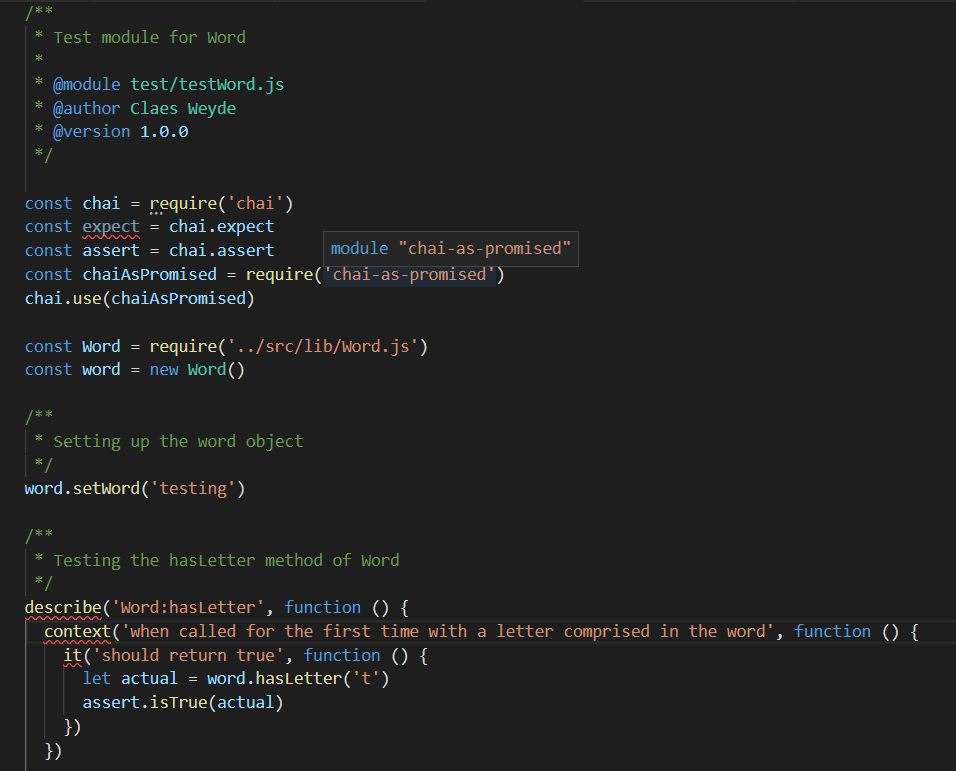
\includegraphics{code3_1}
	\caption{Test code for Word 1 of 2}
	\centering
\end{figure}
\begin{figure}[H]\label{fig:code32}
	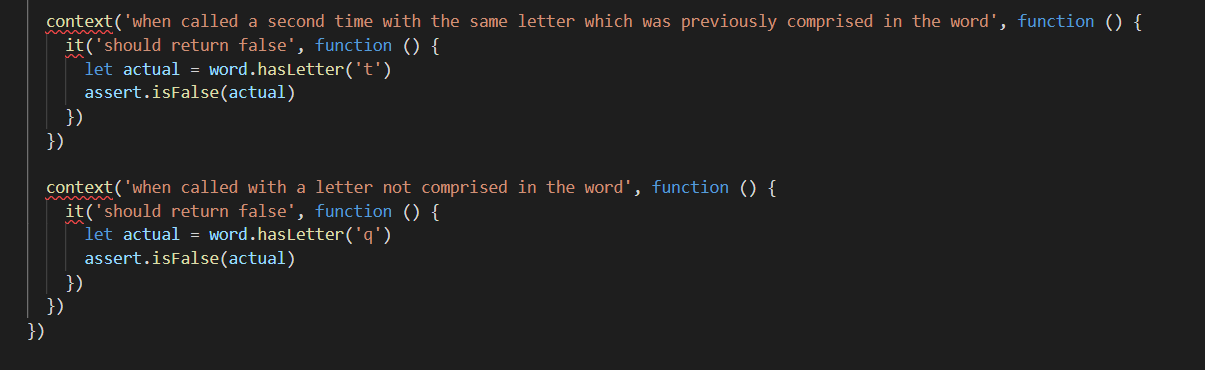
\includegraphics[width=15cm]{code3_2}
	\caption{Test code for Word 2 of 2}
	\centering
\end{figure}
\newpage
\section{Test report for tests}\label{matrix}
\subsection{Manual test matrix}
\begin{center}
	\begin{tabular}{|c|c|c|c|c|c|} 
		\hline
		\textbf{Test} & \textbf{UC 2} & \textbf{UC 4} & \textbf{UC 5} & \textbf{UC 6} & \textbf{UC7} \\ [0.5ex] 
		\hline\hline
		TC 2.2 & 1 & 0 & 0 & 0 & 0 \\
		\hline
		TC 2.3 & 1 & 0 & 0 & 0 & 0 \\
		\hline 
		TC 2.6 & 1 & 0 & 0 & 0 & 0 \\
		\hline 
		TC 2.a* & 1 & 0 & 0 & 0 & 0\\
		\hline
		TC 5.3 & 0 & 0 & 1 & 0 & 0\\ 
		\hline
		TC 5.5 & 0 & 0 & 1 & 0 & 0\\ 
		\hline
		TC 6.2 & 0 & 0 & 0 & 1 & 0\\ 
		\hline
		TC 6.3.1 & 0 & 0 & 0 & 1 & 0\\ 
		\hline
		TC 6.3.2 & 0 & 0 & 0 & 1 & 0\\ 
		\hline
		TC 6.3.2a & 0 & 0 & 0 & 1 & 0\\ 
		\hline
		TC 6.3.2b & 0 & 0 & 0 & 1/Not OK & 0\\
		\hline
		TC 7.3 & 0 & 0 & 0 & 0 & 1\\ 
		\hline
		TC 7.5 & 0 & 0 & 0 & 0 & 1\\ 
		\hline
		TC 7.6 & 0 & 0 & 0 & 0 & 1\\ 		
		\hline
		\textbf{Coverage and success} & 4/OK & 0 & 2/OK & 3/4 OK & 3/OK \\[1ex]
		\hline 
	\end{tabular}
\end{center}
\subsection{Automated test matrix}
\begin{center}
	\begin{tabular}{|c|c|c|c|c|} 
		\hline
		\textbf{Test} & \textbf{Word} & \textbf{Funcs} & \textbf{FileHandler} & \textbf{Authenticator} \\ [0.5ex] 
		\hline\hline
		testWord & 3 & 0 & 0 & 0  \\
		\hline
		testFileHandler & 0 & 0 & 4 & 0  \\
		\hline 
		testAthenticator & 0 & 0 & 0 & 5  \\
		\hline  		
		\hline
		\textbf{Coverage and success} & 3/OK & 0 & 4/OK & 4/OK  \\[1ex]
		\hline 
	\end{tabular}
\end{center}

\begin{center}
	\begin{tabular}{|c|c|c|c|c|} 
		\hline
		\textbf{Test} & \textbf{Game} & \textbf{WordList} & \textbf{HighScores} & \textbf{Player} \\ [0.5ex] 
		\hline\hline
		testWord & 0 & 0 & 0 & 0  \\
		\hline
		testFileHandler & 0 & 0 & 0 & 0  \\
		\hline 
		testAthenticator & 0 & 0 & 0 & 0  \\
		\hline  		
		\hline
		\textbf{Coverage and success} & 0 & 0 & 0 & 0  \\[1ex]
		\hline 
	\end{tabular}
\end{center}
\section{Reflection}
Having performed these tests I believe that testing is not only crucial for finding faults within the code, but also that testing at an early phase will actually make the code better. I believe this is especially true for the unit tests since these made me realize and think more about my actual method implementations, specifically with regards to my inputs and the outputs received. Thus, the code would not only be better because less bugs are found, but also because the code is logical with a good separation of concerns between different components. Continuing forward my goal will be to test early if possible.
\end{document}          
